\chapter{ \label{appendix:normalisation} Normalisation and univariate clustering}

%The aim of this chapter is to give an overview of univariate normalisation methods.
%These methods are illustrated on simulated and real biological datasets.
%These methods can be generalised to multivariate datasets if ind

%The objective of flow cytometry is to capture variation in the biological sample not variation linked to the instrument or to other experimental factors.
%Normalisation is the process of factoring out non-biological for sensible comparison fo samples analysed at different times or on different instruments.

%Generally, samples obtained under controlled conditions should be sufficiently similar and variation in the whole sample is due to experimental artifact.
%Which is why normalisation should be done on the whole sample rather than a subset of the sample.

%The idea follows from gene MA that overall gene expression obtained under similar conditions should be quite similar.
%Hence normalisation in flow cytometry should be done on the whole sample (before any subsetting takes place).

%As datasets get larger they get more similar
%on a large scale things are quite similar but as we dig deeper into subsets distributions look different
%Or that the p-values in a GWAS should follow some empirical distribution.
%We will see that different normalisation approaches make different assumptions about what is unwanted variation.

%\section{Data sets} 
%\paragraph{KIR copy number} 
%\paragraph{Flow data}

\section{Data driven normalisation}


\paragraph{Data dependent normalisation}

In the case of flow cytometry, the distributions are typically multimodal since they are representative of a mixture of cell populations.
The modes of the distributions are representative of how the expected quantity of protein carried on the surface of different cell types which,
in theory, should remain fairly stable if cells are of the same type.
However, the relative frequencies of the cell populations is susceptible to variations in sampling and so is expected to be less stable.
In such a scenario, a reasonable normalisation method is to align the modes i.e the peaks of the distributions so that different cell populations are centered
in a similar location across samples even when their relative quantity changes.
The implementation of this normalisation method then depends on the method used to identify the peaks and to match them across samples.

The best scenario is when the number of peaks is known and constant across samples.
In this scenario, basic clustering algorithms such as k-means or k-medoids, can be applied to identify the peaks in each sample.
Once the peaks have been identified a transform can then be defined so that they are aligned across samples.
If there are only two peaks, a linear transform can perfectly align the two peaks, but if there are more than two peaks, alignement may necessitate a non-linear transform.
%The shifting of the data of the data can be done using a linear transform which scales the variance by the slope squared.

Next let's consider normalisation of multivariate distributions.  
The purpose of principal component correction is to remove unwanted correlation between samples.
When applying a linear transform to multivariate data the correlation between the dimensions is preserved since the multiplicative factors cancel out.
However the covariance changes.
Care must be taken when applying a non-linear transform.  
Normalisation is effectively analogous to meta-clustering since we are attempting to match cell populations across samples.  
Normalisation facilitates matching clusters across datasets but in doing can remove meaningful biological variation.  
A less biased approach is to allow for different cluster location and shapes across datasets and instead incorporate the clustering in some sort of hierarchical framework.  
Normalisation or meta-clustering is a necessary step when data is pooled across studies.



Perhaps the most basic form of normalisation is scaling: we substract the mean and divide by the variance so that the resulting distribution has a mean of zero and a variance of one.
%This approach is sensible if the distibutions are symmetric unimodal like the normal distribution.
Figure~\ref{normalisation-scaled} is a trivial example of scaling on simulated data.
%$x_0 \sim N

%% Scaling
\begin{figure}[ht]
\begin{subfigure}[b]{.5\textwidth}
\centering
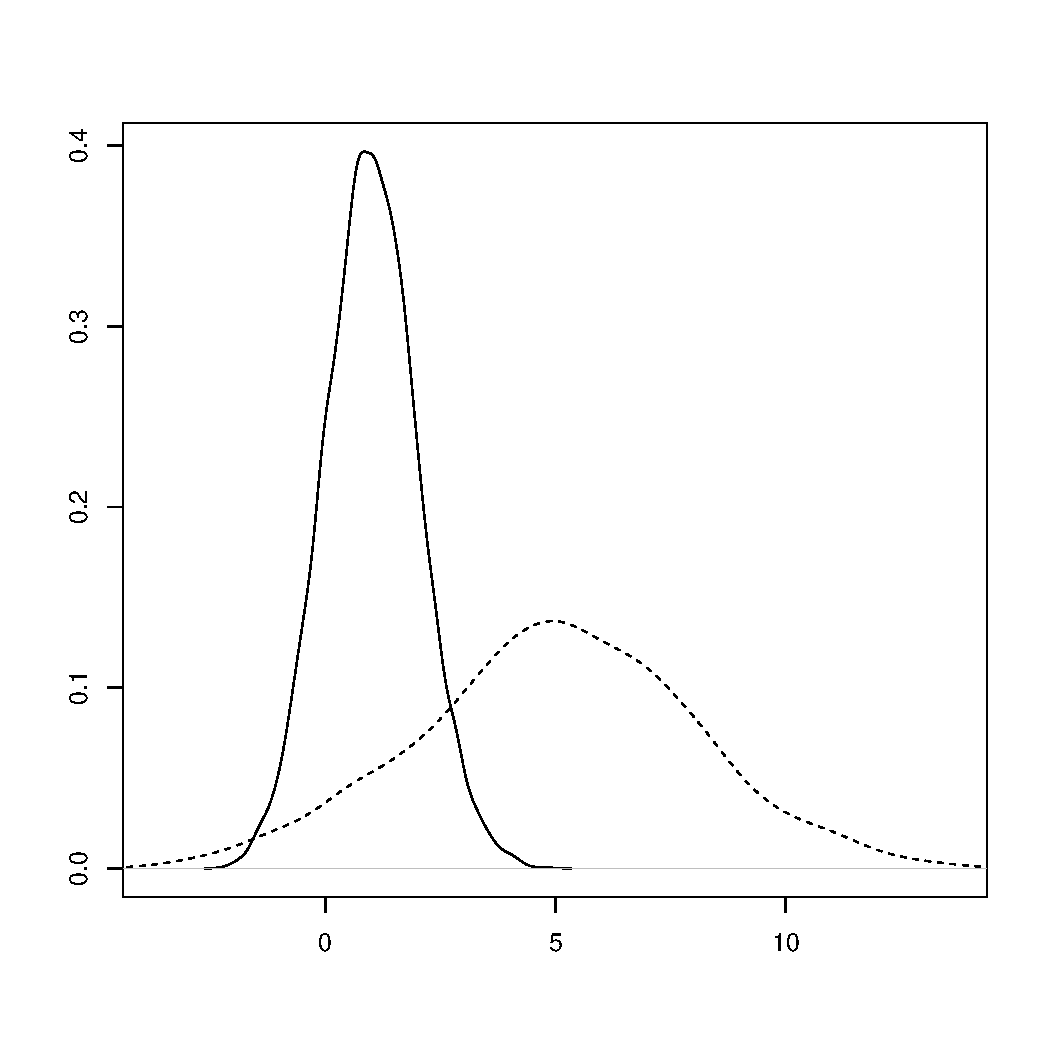
\includegraphics[scale=.4]{figures/normalisation-scaled-a.pdf} 
\caption{before scaling}
\end{subfigure}
~
\begin{subfigure}[b]{.5\textwidth}
\centering
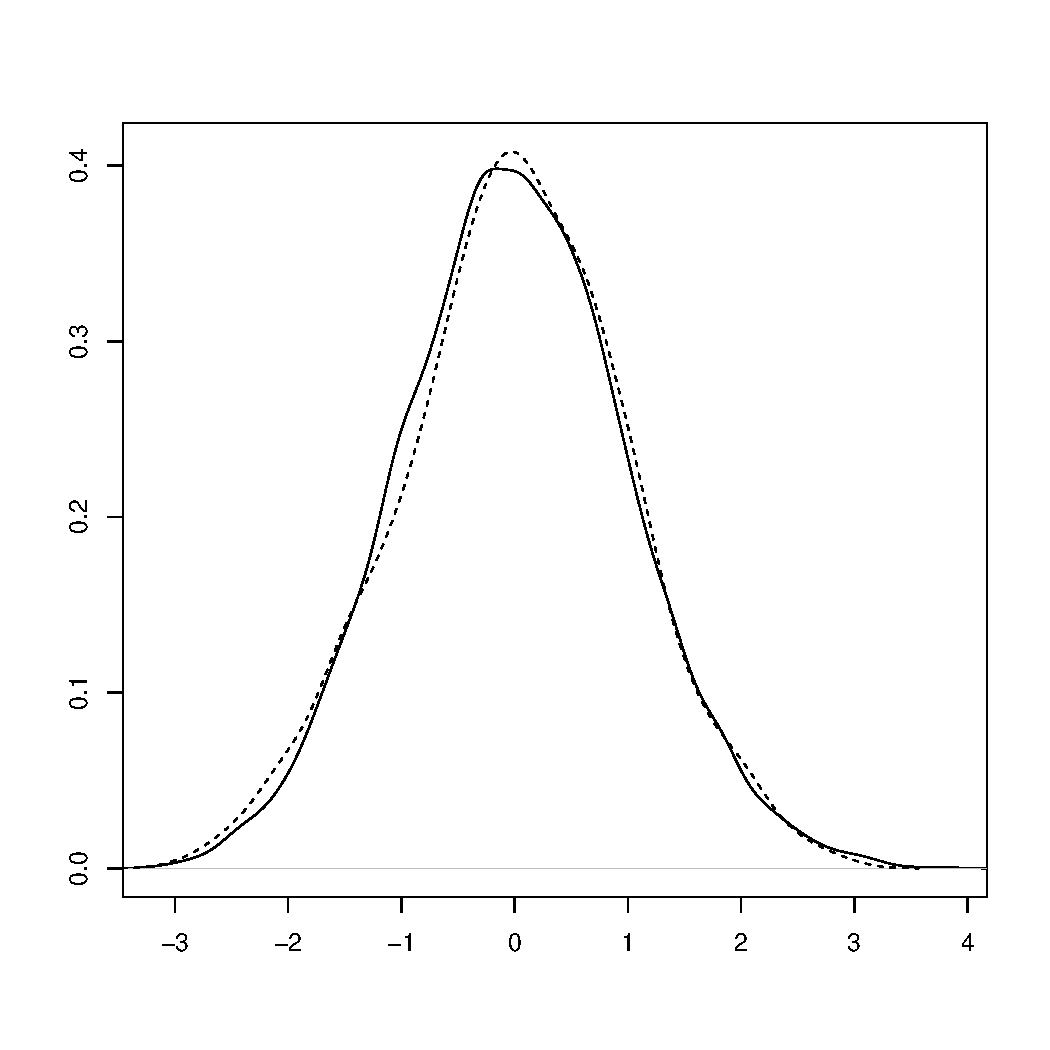
\includegraphics[scale=.4]{figures/normalisation-scaled-b.pdf} 
\caption{after scaling}
\end{subfigure}
\mycaption{normalisation-scaled}
{Normalisation by scaling on simulated data.}
{
In solid black line represents the density function obtained from $10,000$ draws from a normal distribution
with with means $\mu_0=1$ and standard deviation $\sigma_0=1$.
The dashed line represents the density function obtained from $1,000$ draws from a normal distribution
where $\mu_1=5$ and $\sigma_1=3$.
After scaling both distributions have $\mu=0$ and $\sigma=1$.
}
\end{figure}


If the distributions are unimodal but not symmetric, such as $\chi^2$ distributions, then an alternative is quantile normalisation.
As can be seen in Figure~\ref{normalisation-quantile}, the quantiles of the distribution are identified
then a transform is applied so that quantiles of one distribution are aligned with those of the other.
Here the transform is a simple linear regression.
Quantile normalisation works well when the shape of the distributions is the same and only shifted.

%% Quantile
\begin{figure}[ht]
\begin{subfigure}[b]{.5\textwidth}
\centering
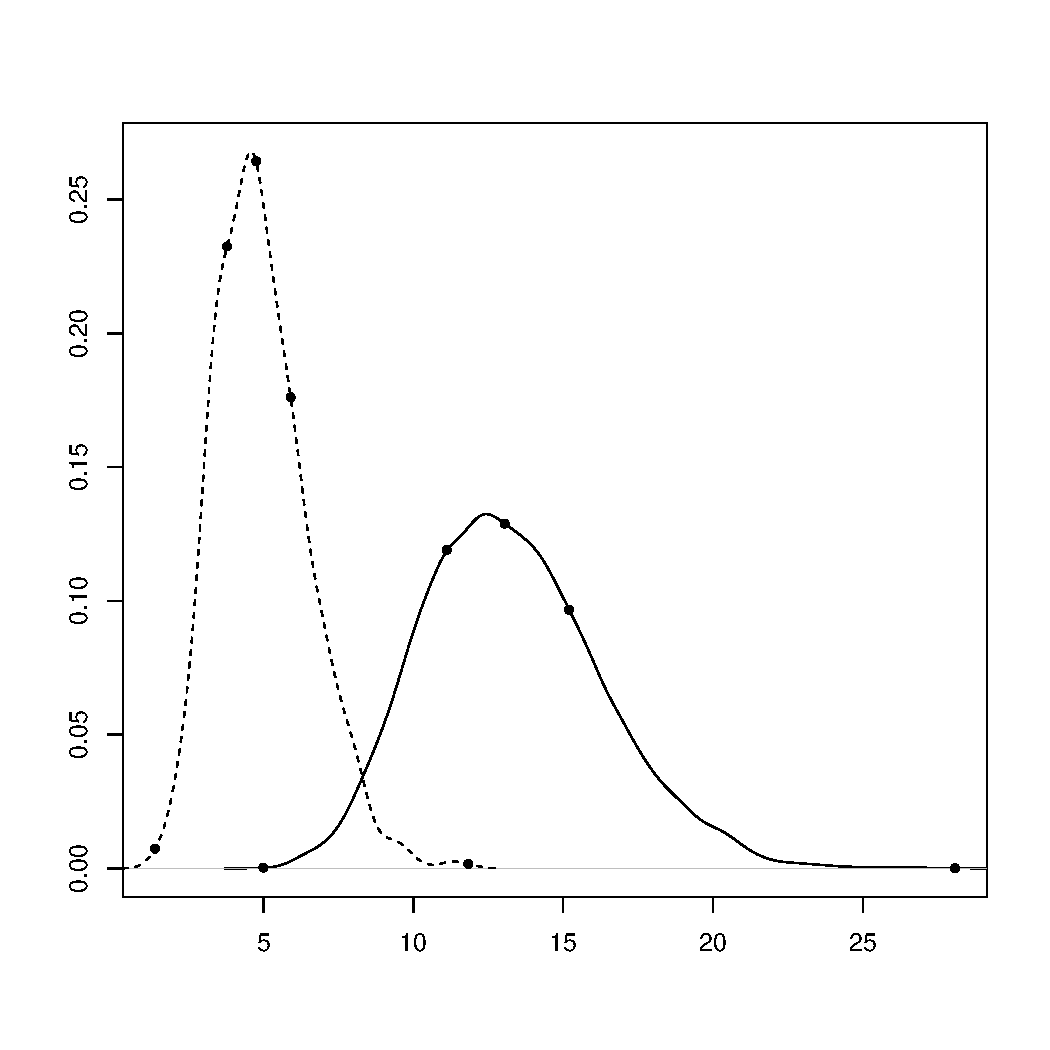
\includegraphics[scale=.4]{figures/normalisation-quantile-a.pdf} 
\caption{before aligning quantiles}
\end{subfigure}
~
\begin{subfigure}[b]{.5\textwidth}
\centering
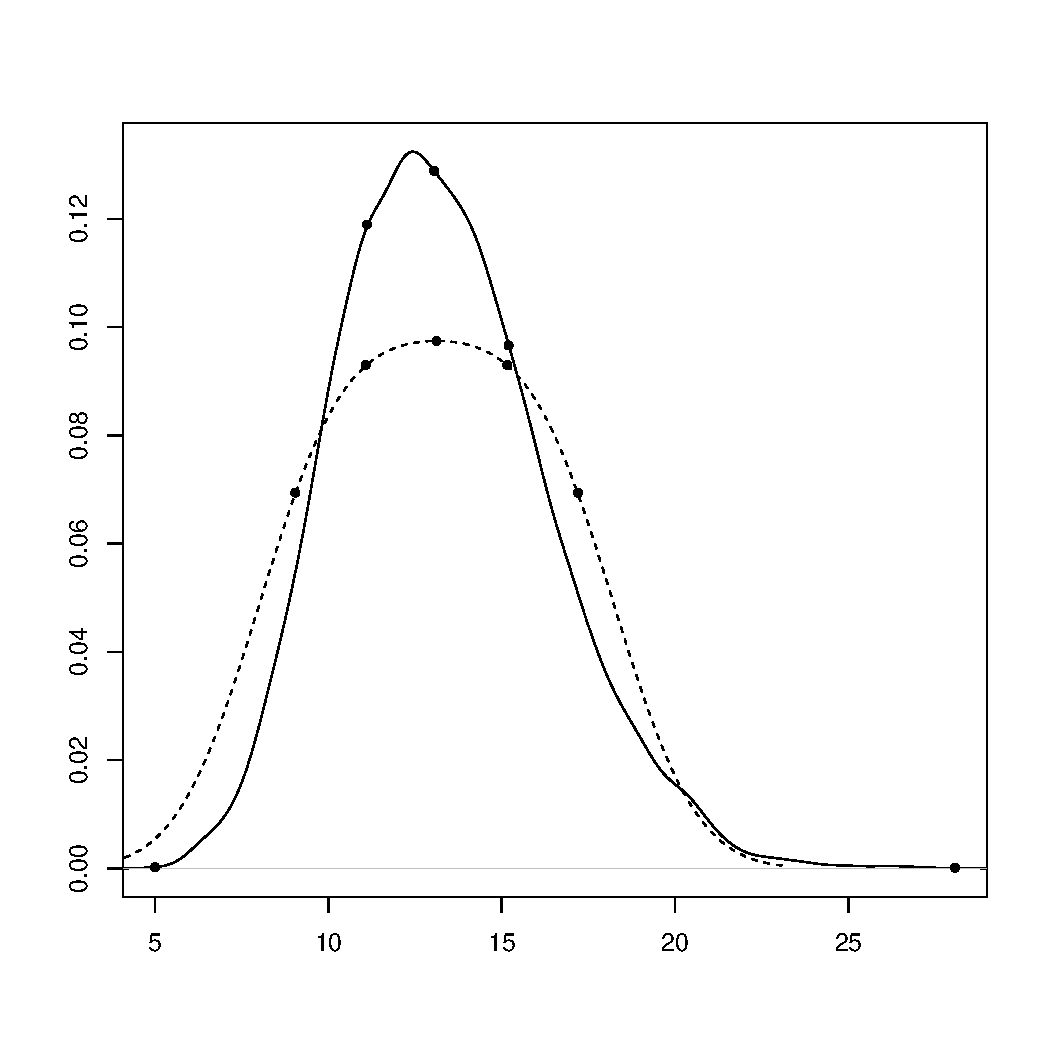
\includegraphics[scale=.4]{figures/normalisation-quantile-b.pdf} 
\caption{after aligning quantiles}
\end{subfigure}
\mycaption{normalisation-quantile}
{Normalisation by quantile alignment on simulated data.}
{
In solid black line represents the density function obtained from $10,000$ draws from a gamma distribution
with with shape $\alpha_0=20$ and rate $\beta_0=1.5$.
The dashed line represents the density function obtained from $1,000$ draws from a gamma distribution
where $\alpha_1=10$ and $\beta_1=2$.
The black dots are the quantiles.
The normalisation finds a linear mapping of the quantiles of the dashed-line distribution onto those of the solid-line distribution.
}
\end{figure}


In real datasets however, univariate distributions are typically multimodal since they contain of a mixture of groups.
In the case of flow cytometry data, the groups are cell populations, and the modes of the distributions, esentially peaks in the density function,
represent the protein quantity carried on the surface of different cell types.
In theory, the locations of these peaks should remain fairly stable across samples provided experimental parameters are kept constant.
Though, in practise there is variation attributed to factors which are beyond our control such as long-term instrument deterioration.
On the other hand, the height of the peaks, the relative frequencies of the cell populations, are expected to change since they are
are susceptible to variation.
%In the case of qPCR data, the groups are reprentative of the copy numbers.

In such a scenario, a reasonable normalisation method is to align the peaks of the distributions so that different cell populations are centered
in a similar location across samples even when their relative quantity changes.
The implementation of this normalisation method then depends on the method used to identify the peaks and to match them across samples.

The ideal scenario is when the number of peaks is known and constant across samples.
This is the case when dealing with synthetic data such as beads.
In this scenario, basic clustering algorithms such as k-means or k-medoids, can be applied to identify the peaks in each sample.
This is the method used by the \Rpackage{flowBeads} BioConductor package which identifies bead populations with the k-medoids algorithm
for the purpose of fluorescence normalisation.

Unfortunately, on real data, the uncontrolled variation between biological samples means that the certain peaks are not consistently identifiable across all samples.
The number of peaks is unknown and can vary between samples. 
More flexible peak searching algorithms are requied to allow for this per sample-variation.

Instead of clustering, another method is to identify peaks in the density function with a sliding window approach.
The sliding window approach records the point with the highest density estimate in the current window.
As a result returning a list of highest density points of which the top K may be chosen.
This is one of the approaches implemented in the \Rpackage{flowStats} BioConductor package.
Here's an example of this method applied on flow data where two common groups stand out and are reasonably well separated (Figure~\ref{figure:normalisation-peaks}).

Sometimes it may be preferable to identify only the most distinguishable subset of peaks, those representative of the most common groups.
This is the method we applied on qPCR data to align common copy number groups 1 and 2 across plates.
%However peaks are not always easily identifiable.


%% Peaks
\begin{figure}[ht]
\begin{subfigure}[b]{.5\textwidth}
\centering
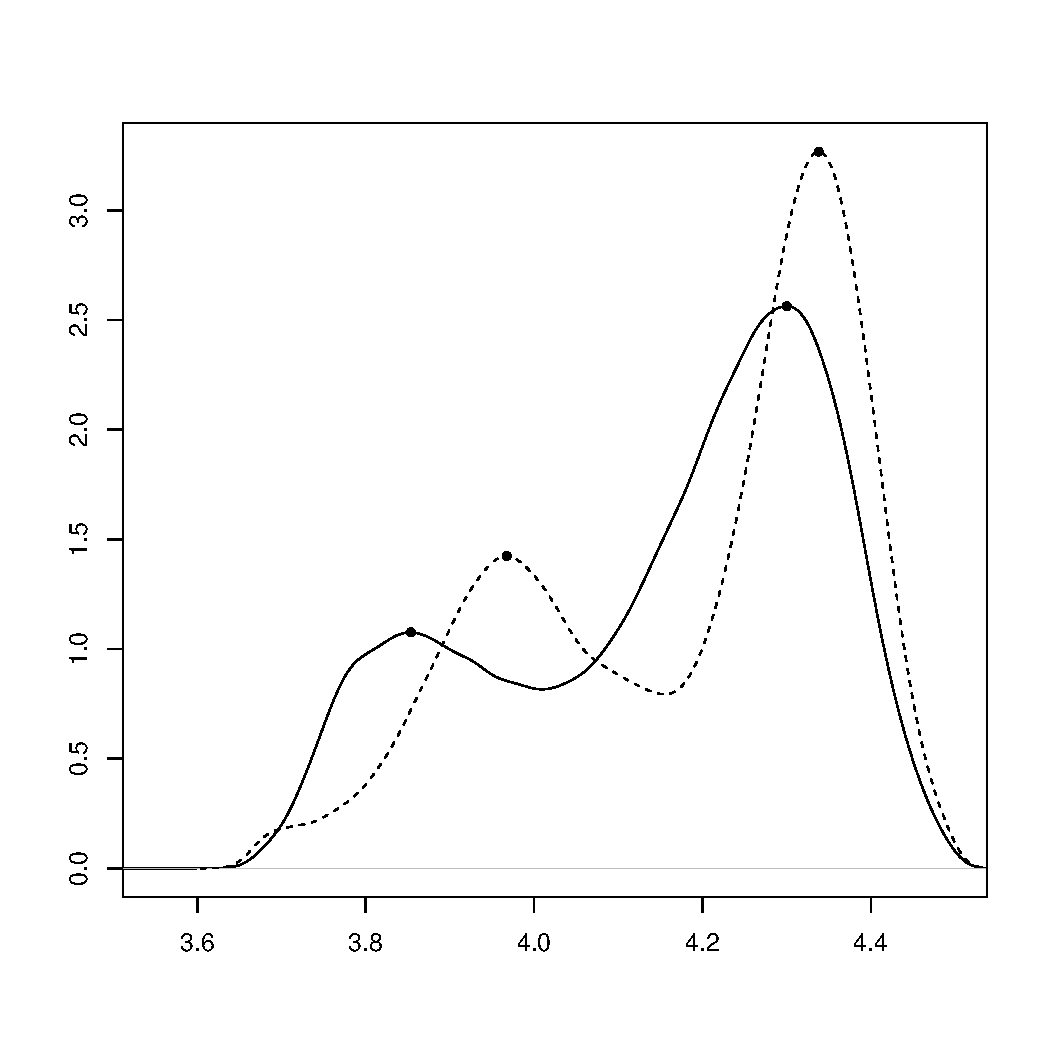
\includegraphics[scale=.4]{figures/normalisation-peaks-a.pdf} 
\caption{identification of peaks}
\end{subfigure}
~
\begin{subfigure}[b]{.5\textwidth}
\centering
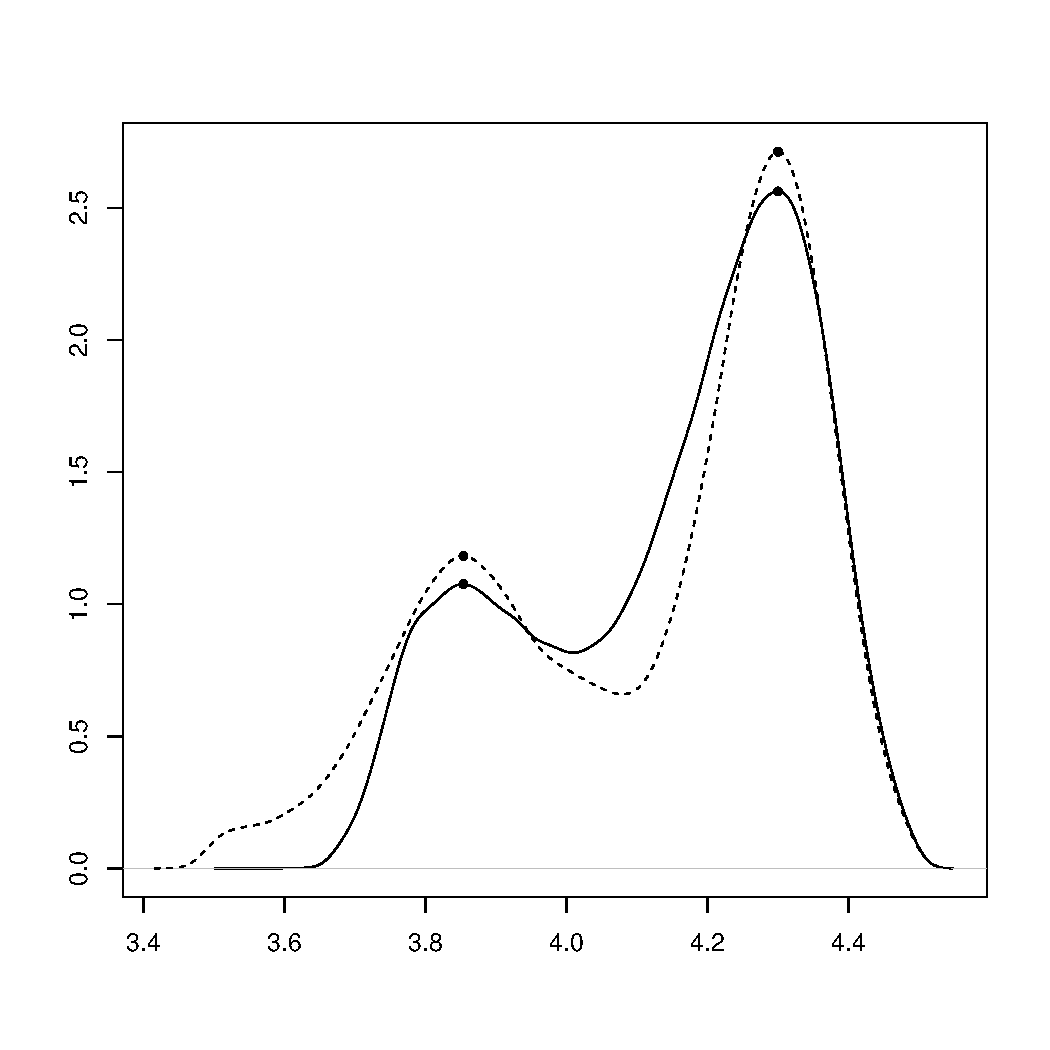
\includegraphics[scale=.4]{figures/normalisation-peaks-b.pdf} 
\caption{peak alignment}
\end{subfigure}
\mycaption{normalisation-peaks}
{Normalisation by peak alignment.}
{
Alignment of the two identified peaks.
}
\end{figure}


These break down into three steps.
First feature are identified within each sample.
Then the features are matched across samples.
Finally the features are aligned across samples using a transform which
may be linear on non-linear.
This last step represents the actual normalisation step.

\subsection{Identification of features within a sample}

Feature identification can work directly on the data, by doing clustering,
or on the shape of the univariate density function.  
The shape and smoothness of the density function is determined by the choice of bandwidth.
Hence these methods which work directly on the density function are sensitive to the bandwidth selection (also known as the smoothing parameter).

\textbf{Sliding-window on the density function}
In the sliding-window approach, when the maximum of the window coincides with the central data point of the window, 
this data point is assigned to be the maximum.
This is the approach adopted by the \Rfunction{guaussNorm} function in \Rpackage{flowStats}.
This method is dependent on the span of the sliding-window.
Peaks are also scored depending on their height and peakness.
This allows for a ranking of the peaks by quality.
I have applied this sliding-window method with a fixed window size of 40 to all three available flow datasets in Figure~\ref{figure:IL2-density-peaks},
Figure~\ref{figure:IL2RA-density-peaks} and Figure~\ref{figure:DILT1D-EFF-density-peaks}.
No attempt has been done to rank the peaks by score, instead the peaks are ordered by their location.
The coloured points represent the peaks identified in each sample.
The colours determine the ordering of the peaks: black, red, green, blue, light-blue.
The success of the peak identification varies greatly between channels.
When the number of peaks identified is not consistent, we see a mixing of the colours.
Sometimes a consensus can be determined from considering all sample.
For example for CD4 in Figure~\ref{figure:IL2-density-peaks}, it is clear
that the correct number of peaks in the majority of samples should be four even when sometimes the first peak is not consistently detected
in a few sample.
On the other hand, in CD45RA of the same figure, it is unclear whether there should be two or three peaks.
Here we might try to use the score of the peaks to decide of where the should peak should lie.


\begin{figure}[h]
  \centering
  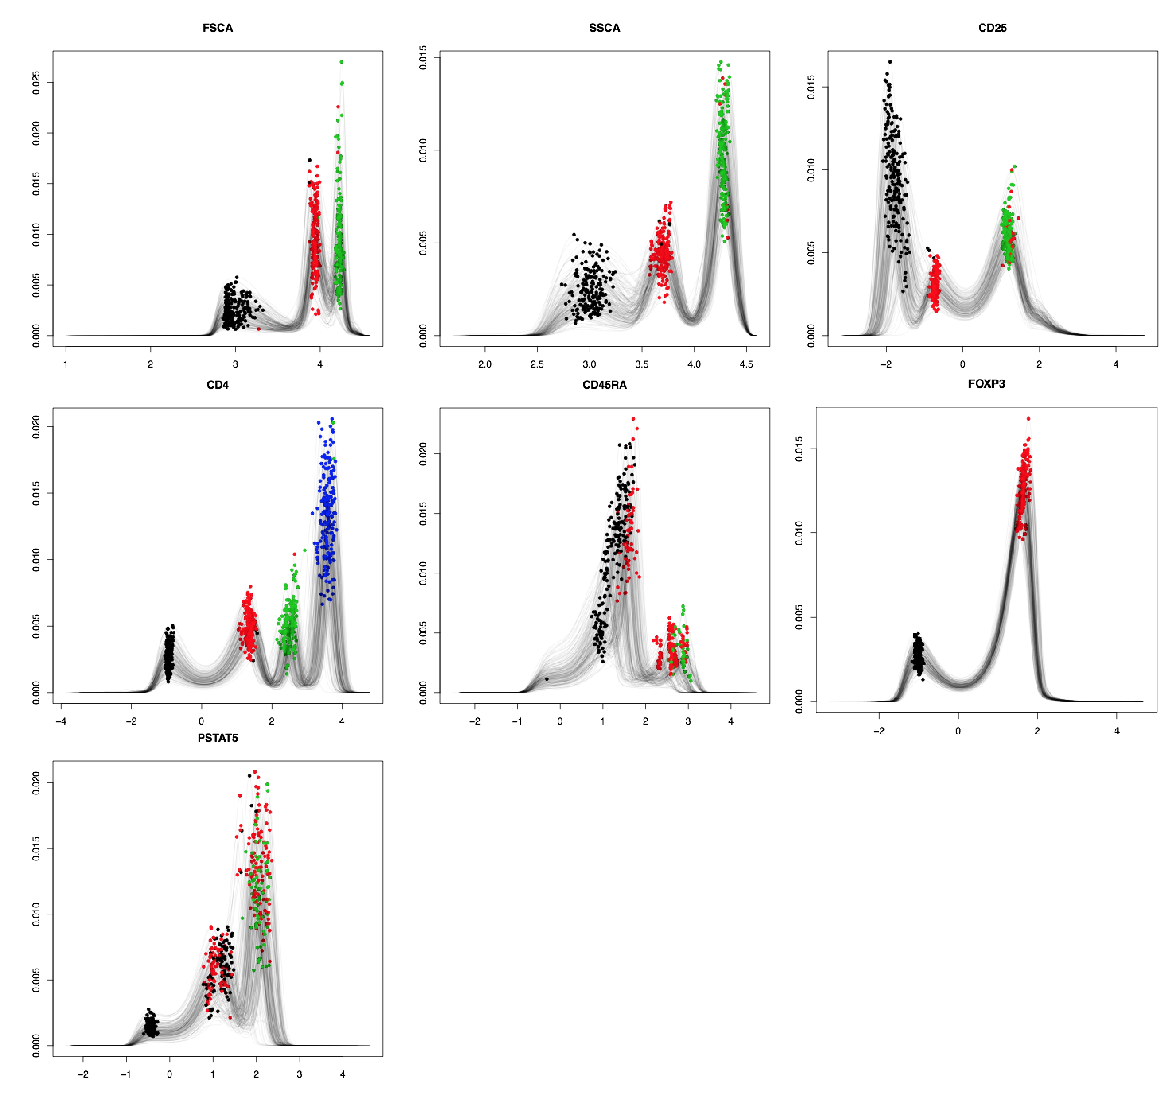
\includegraphics[scale=.75]{figures/IL2-density-peaks.pdf}
  \mycaption{figure:IL2-density-peaks}{IL-2 stimulation dataset, sliding-window span $40$.}{  
  The coloured points indicate the peaks as identified by the sliding window approach with a window span of 40.
  The colouring indicate the number of the peak. The respective ordering for four peaks is black, red, green, blue.
  Notice that often there is mixing of the colours.
  This happens because the same number peaks is not always identified depending on the sample and window size.
  In fact certain peaks can not be reliably identified such as on pSTAT5.
}
\end{figure}


\begin{figure}[h]
  \centering
  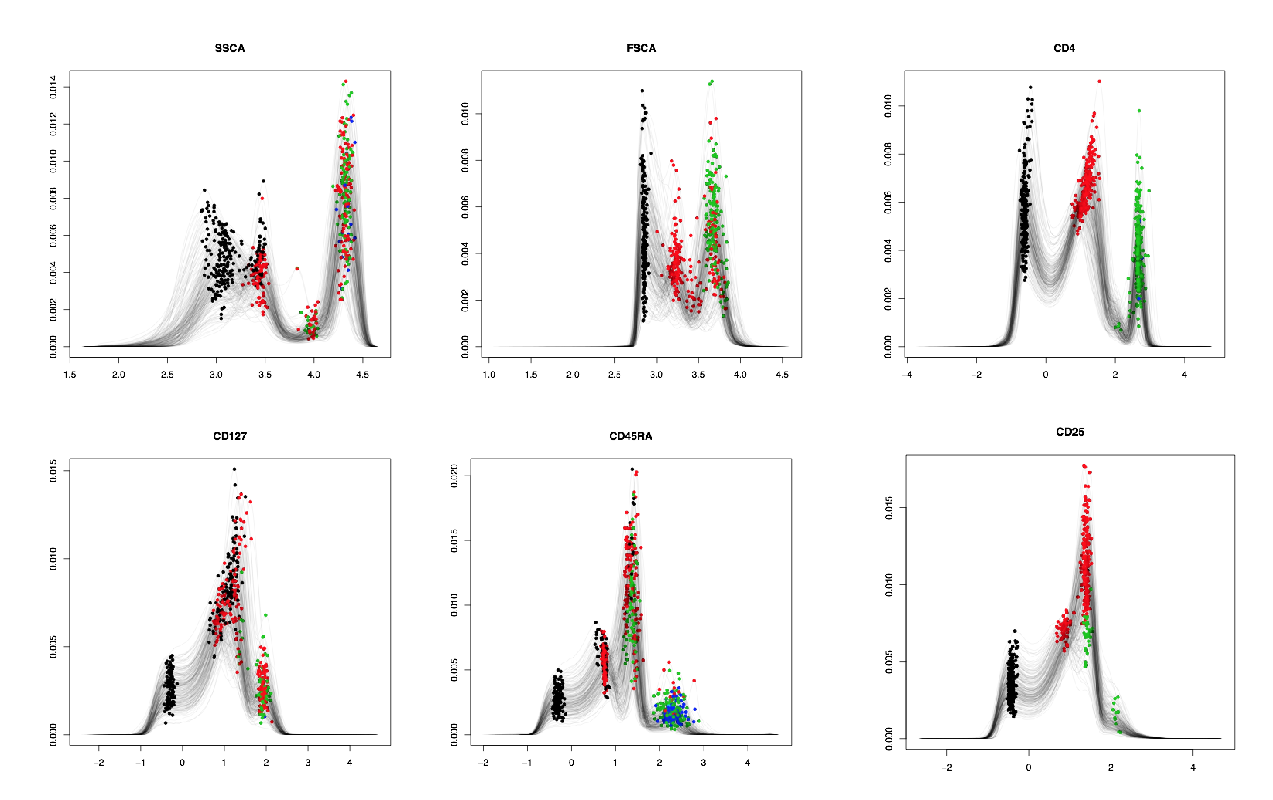
\includegraphics[scale=.75]{figures/IL2RA-density-peaks.pdf}
  \mycaption{figure:IL2RA-density-peaks}{IL2RA dataset, sliding-window span $40$.}{
  The coloured points indicate the peaks as identified by the sliding window approach with a window span of 40.
  The colouring indicate the number of the peak. The respective ordering for four peaks is black, red, green, blue.
  Notice that often there is mixing of the colours.
  This happens because the same number peaks is not always identified depending on the sample and window size.
  In fact certain peaks can not be reliably identified such as on pSTAT5.
  }
\end{figure}


\begin{figure}[h]
  \centering
  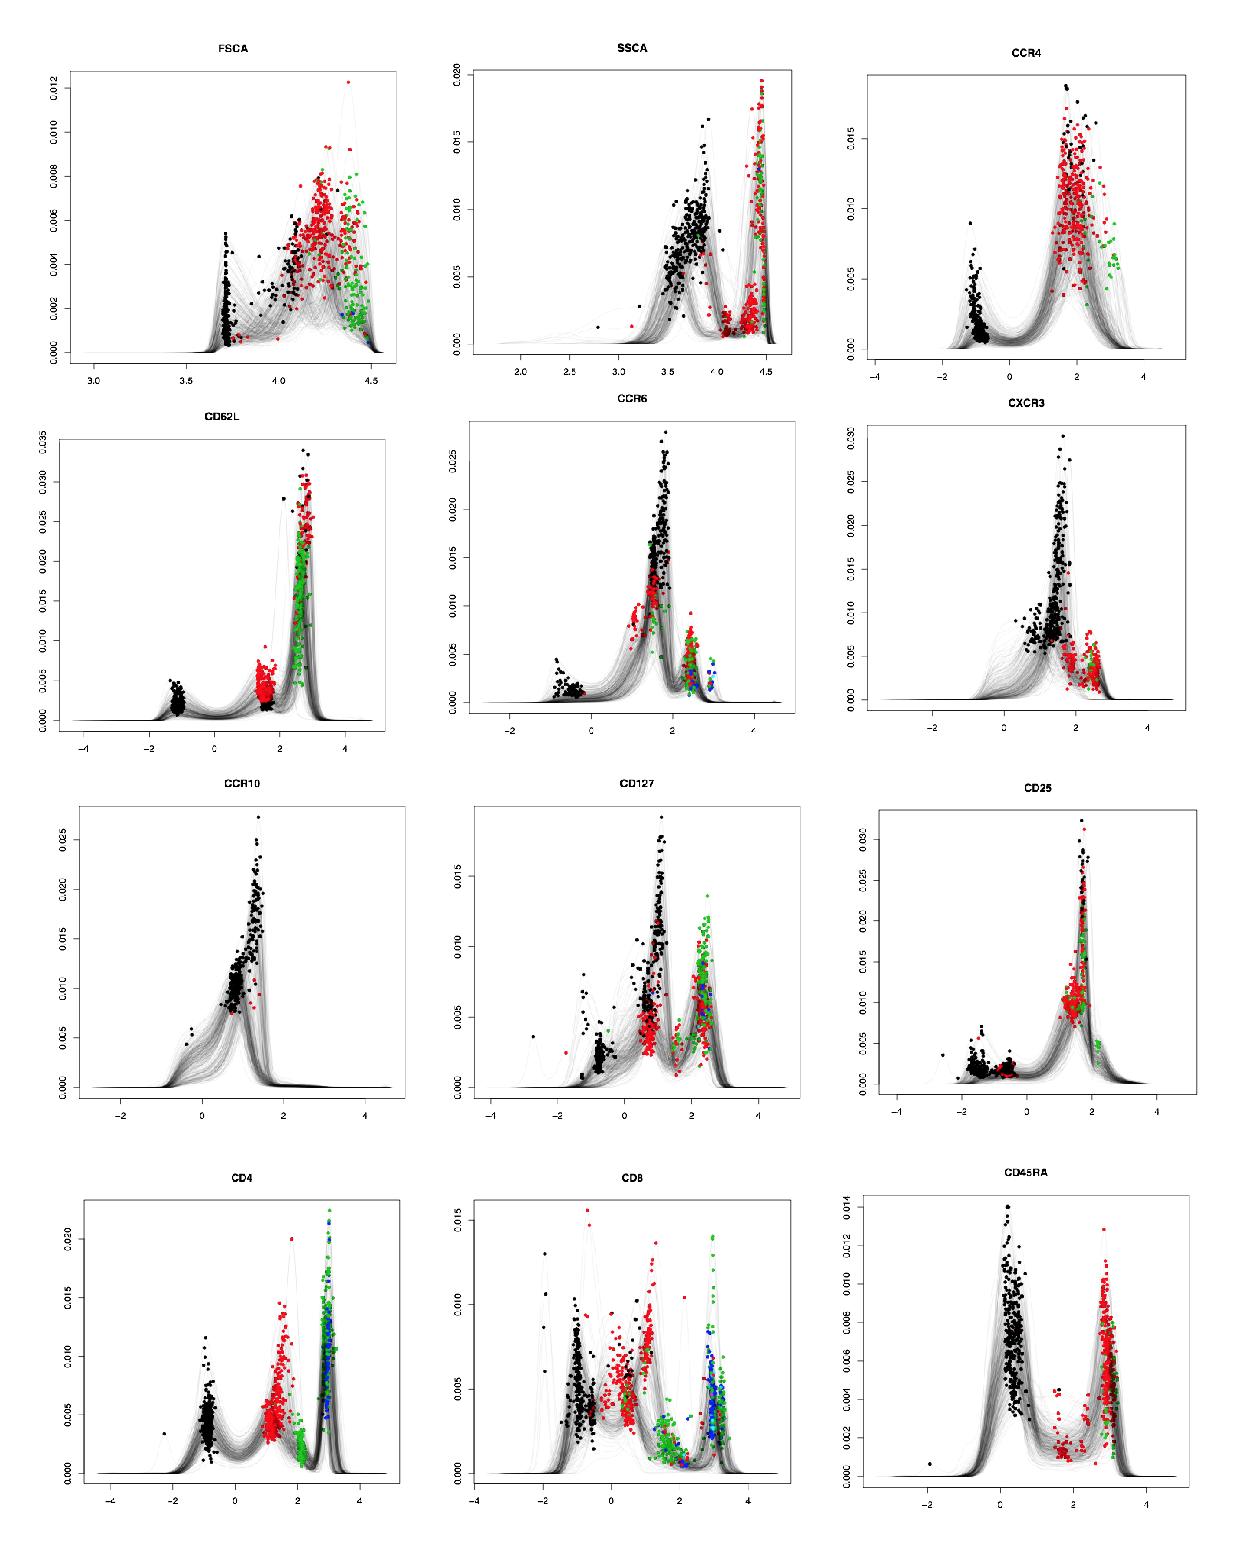
\includegraphics[scale=.75]{figures/DILT1D-EFF-density-peaks.pdf}
  \mycaption{figure:DILT1D-EFF-density-peaks}{DILT1D dataset, sliding-window span $40$.}{
  The coloured points indicate the peaks as identified by the sliding window approach with a window span of 40.
  The colouring indicate the number of the peak. The respective ordering for four peaks is black, red, green, blue.
  Notice that often there is mixing of the colours.
  This happens because the same number peaks is not always identified depending on the sample and window size.
  In fact certain peaks can not be reliably identified such as on pSTAT5.
}
\end{figure}


\clearpage


\paragraph{Feature signifance of the density function}

%The reliance on the bandwidth by trying a selection of bandwidths.
Another approach is to estimate feature significance using the gradient and curvature kernel density estimation \citep{Chaudhuri:1999gu,Duong:2008eu}.
%SiZer: significant zero crossing of derivatives

This approach as implemented by \Rfunction{featureSignif} in the \Rpackage{feature} R package, relies on a $\chi^2$ significance test.

Feature identification uses the first (gradient) and second derivate (curvature) of the density function to identify features such as local maxima, minima or points of inflection.
Local maxima are points where the first derivative is zero and the second derivative is strictly negative.
Local minima are ponts where the first derivative is zero and the seoncd derivative is strictly positive.
%When both the first and second derivative are zero then it's a point of inflection.

In practise however this method does not reliably identify peaks.
Possibly, the bandwidth and threshold significance threshold selection require better estimation.


\paragraph{Clustering}
Peaks in the density function can be also identified without explicitly analysing the density function but instead by using data clustering.
These methods are sensitive to the number of clusters parameters which, as mentionned, may not always be consistently identifiable across samples.
Perhaps the number of cluster can be estimated from the sliding window results obtained on all samples.

The most fundamental and well known univariate clustering algorithm is K-means (see Appendix\ref{appendix:clustering}).


\subsection{Feature matching across samples }

Feature matching, also called feature registration, attempts to match the identified features across samples.
This is similar to a meta-clustering step.
Samples may have different number of features.
Density features can be matched on properties such location and height.
Clusters can be matched using position or size of group.
Consensus about the number of groups common to all samples.


\subsection{Alignment of features across samples}

Methods which attempt to align the features/landmarks of the density functions via some linear or non-linear transform \citep{Hahne:2009hl}.

Once the peaks have been identified a transform can then be defined so that they are aligned across samples.
If there are only two peaks, then a linear transform perfectly aligns the two peaks.
But if there are more than two peaks, alignment could necessitate a non-linear transform.
However this runs the risk of introducing too much extra-variation in the dataset.
%The shifting of the data of the data can be done using a linear transform which scales the variance by the slope squared.

\paragraph{Linear}

Linear regression preserves variance.
But certain peaks which are far from the mean have more leverage.
Peaks may be weighted by their height, since more significant should be attributed more weight.


\paragraph{Non-linear}

In the \Rpackage{flowStats}, two methods non-linear are suggested: \Rfunction{gaussNorm} and \Rfunction{fdaNorm}.

In the \Rfunction{gaussNorm} approach, the amount by which the data points are shifted is exponentially decreased as the points are further away from the features.
Thus features can be moved independently from each other.

In the \Rfunction{fdaNorm} approach, after approximating the density function with b-splines and identifying features, a warping function is used to transform the curves.
This is also known as curve registration and is implemented in the fda R package.

Another non-linear regression approach is local regression.

The loess approach uses locally weighted polynomial

At each point in the data set a low-degree polynomial is fitted to a subset of the data, with explanatory variable values near the point whose response is being estimated.
The polynomial is fitted using weighted least squares, giving more weight to points near the point whose response is being estimated and less weight to points further away.
The value of the regression function for the point is then obtained by evaluating the local polynomial using the explanatory variable values for that data point.
The loess fit is complete after regression function values have been computed for each of the n data points.

Many of the details of this method, such as the degree of the polynomial model and the weights, are flexible.


%\begin{figure}[h]
%%
%%#simulated data
%%x0 <- mixtools::rnormmix(1000, mu=c(1,6), lambda=c(.3,.7))
%%x1 <- mixtools::rnormmix(1000, mu=.9*c(1,6)+2, lambda=c(.5,.5), sigma=c(2,2))
%%d0 <- density(x0)
%%d1 <- density(x1)
%%l0 <- extract.landmarks(x0,max.lms=2, bw=d0$bw)
%%l1 <- extract.landmarks(x1,max.lms=2, bw=d1$bw)
%%m <- lm(l0$lms ~ l1$lms)
%%x1.norm <- cbind(1,x1)%*%coefficients(m)
%%l1.norm <- extract.landmarks(x1.norm,max.lms=2)
%%#before align
%%pdf('~nikolas/GoogleDrive/PhD/Thesis/IL2/figures/simulation-peak-align-noise.pdf')
%%plot(d0,xlim=c(-3,11),main='', xlab='')
%%points(l0$lms, l0$dens, pch=20, cex=2)
%%lines(d1, lty=2)
%%points(l1$lms, l1$dens, pch=20, cex=2)
%%#after peak align
%%lines(density(x1.norm), lty=2, col='red')
%%points(l1.norm$lms, l1.norm$dens, pch=20, cex=2, col='red')
%%dev.off()
%%
    %\centering
    %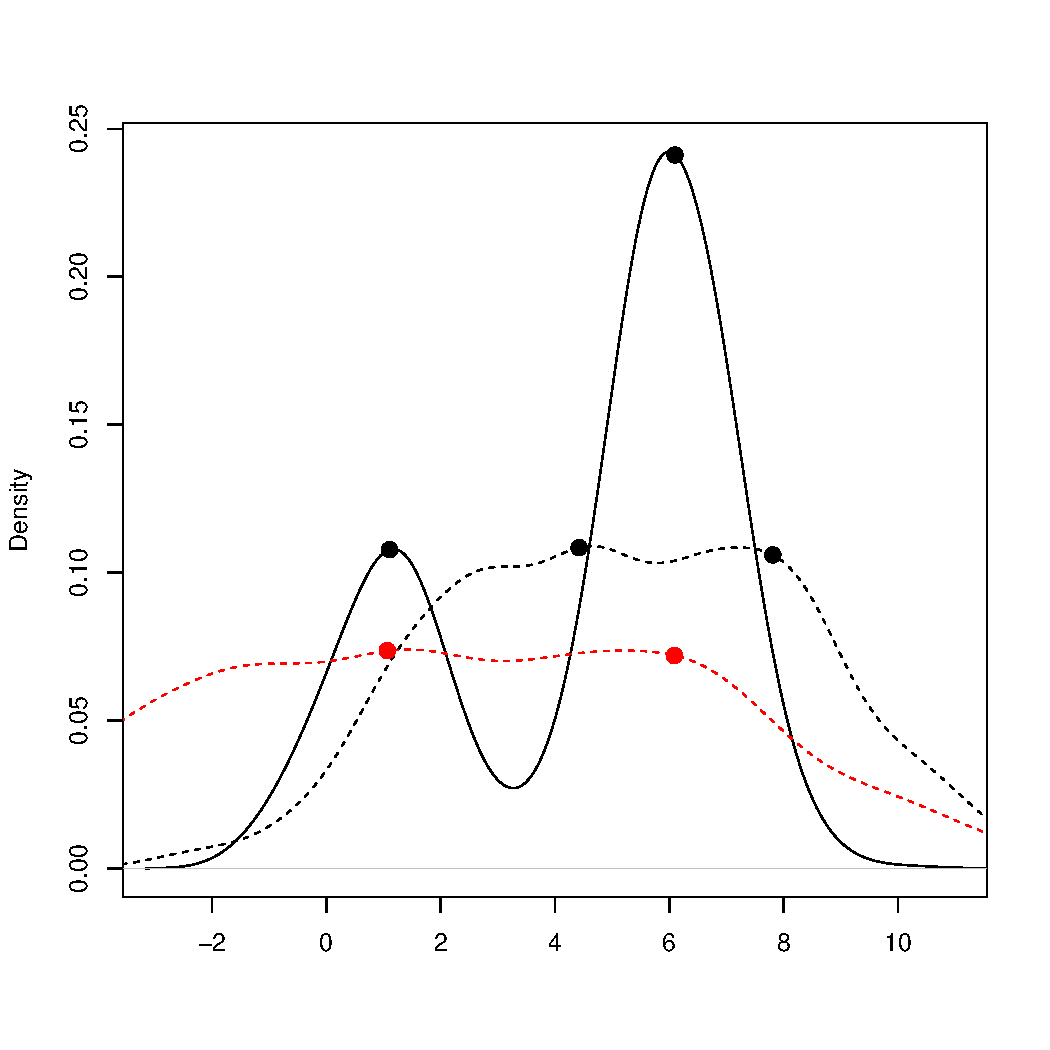
\includegraphics[scale=1]{IL2/figures/simulation-peak-align-noise.pdf}
    %\caption{  \label{figure:simulation-peak-align-noise}  In solid black line represents the density function obtained from $1000$ draws from a mixture of two normal distribution
    %with means $\mu_0=(1,6)$, standard deviations $\sigma_0=(1,1)$ and mixing proportions $\tau_0=(.3,.7)$.
    %The dashed black line represents the density function obtained from $1000$ draws from a mixture of two normal distribution
    %where $\mu_1 = 0.9 \mu_0 + 2$, standard deviations $\sigma_0=(1,1)$ and $\tau_1=(.5,.5)$.
    %The red dashed line represents the transformation using peak alignment. }
%\end{figure}
%



\section{Normalisation with controls}

The normalisation methods considered so far are data only.
However often, little is known of the data being analysed and prior knowledge can bias our analysis.
When available internal (spike-ins) or external controls, can yield a less biased normalisation technique.
Instrument variation can be detected by using a synthetic object of known and stable property which can be analysed within the sample
or independently.
In flow cytometry, fluorescent beads can be used to make intensity data comparable across days.
This method is described in Chapter 1.


